\documentclass[12pt,a4paper]{article}

\usepackage[utf8]{inputenc}
\usepackage[T2A]{fontenc}
\usepackage[ukrainian]{babel}
\usepackage{geometry}
\geometry{
    left=2cm,
    right=2cm,
    top=2cm,
    bottom=2cm
}

\usepackage[table]{xcolor}
\usepackage{amsmath}
\usepackage{graphicx}
\usepackage{subcaption}
\usepackage{multirow}
\usepackage{makecell}
\usepackage{pdflscape}
\usepackage{array}
\usepackage{fancyvrb}
\newcolumntype{C}[1]{>{\centering\arraybackslash}m{#1}}

\usepackage{minted}

\usemintedstyle{vs}
\setminted{linenos, breaklines, frame=single, fontsize=\small}

\RecustomVerbatimCommand{\VerbatimInput}{VerbatimInput}{
    breaklines=true,
    breaksymbolleft={}
}

\usepackage[
  unicode,
  pdftitle={ІО-41, Давидчук А.М., Цифрова схемотехніка, Лабораторна робота №6},
  pdfauthor={Давидчук Артем},
  pdfsubject={Цифрова схемотехніка}
]{hyperref}

\begin{document}

    \hypersetup{pageanchor=false}
    \begin{titlepage}

        \begin{center}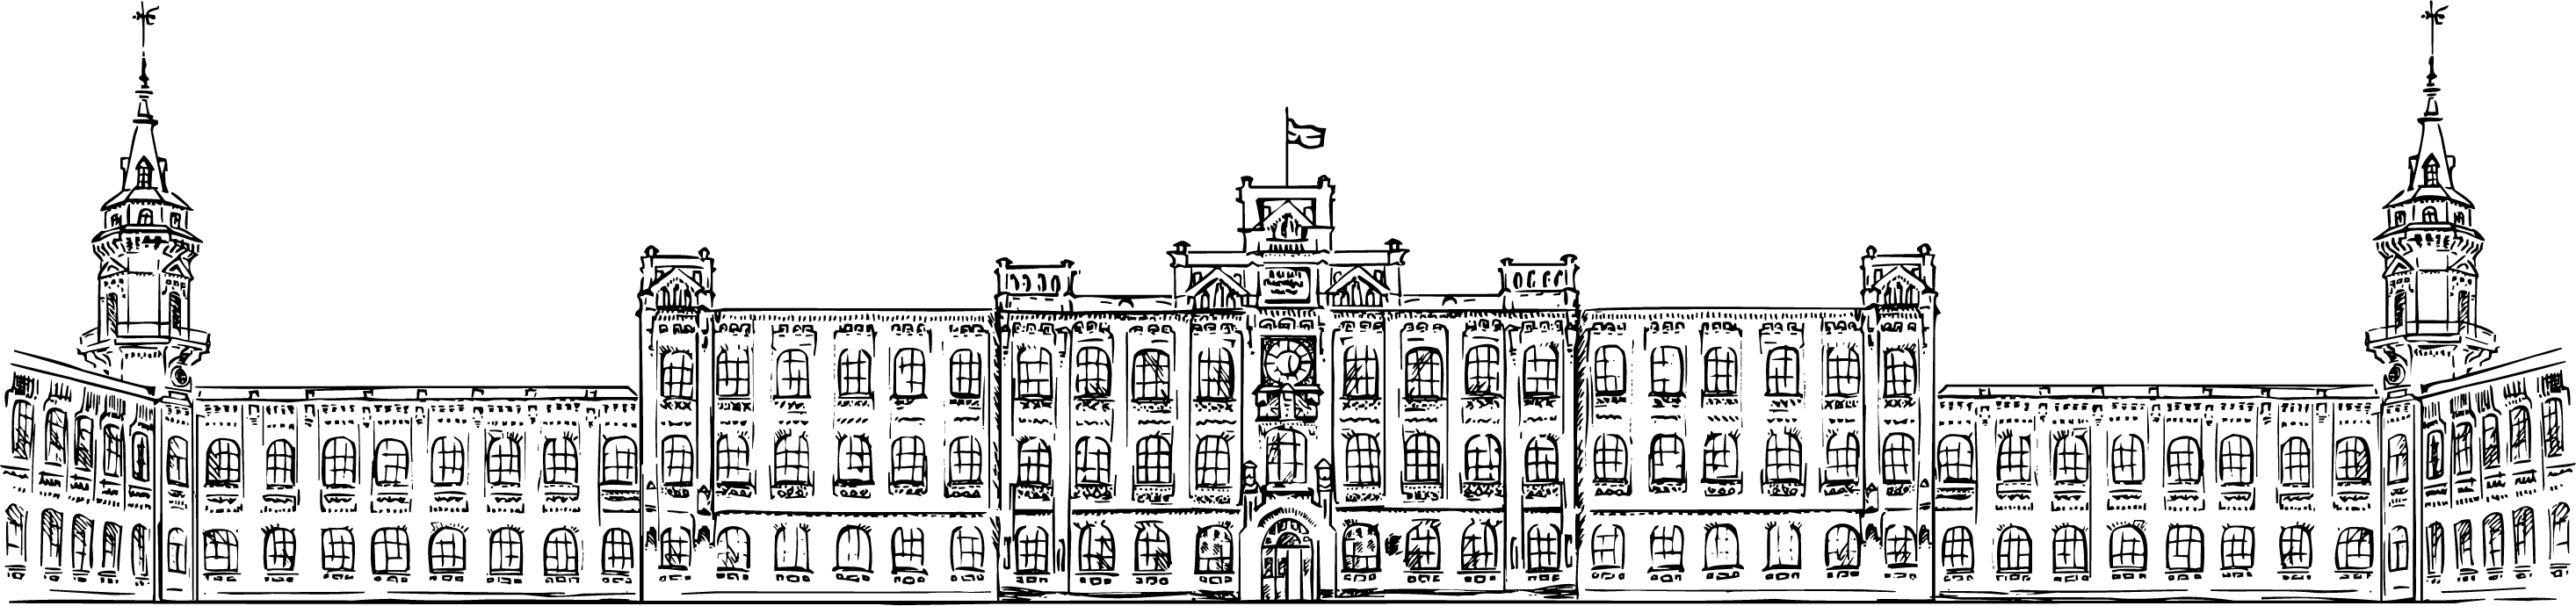
\includegraphics[width=0.7\textwidth]{../../../TITLES/letterhead.png}\end{center}

        \begin{center}
            \large Національний технічний університет України\\
            «Київський політехнічний інститут імені Ігоря Сікорського»\\[1em]
            Факультет інформатики та обчислювальної техніки\\
            Кафедра обчислювальної техніки
        \end{center}

        \vfill

        \begin{center}
            \textbf{\LARGE Цифрова схемотехніка}\\[2em]
            \textbf{\Large Лабораторна робота №6}\\[0.5em]
            «Пристрої для перетворення чисел. Типові вузли комп'ютера»
        \end{center}

        \vfill

        \begin{flushright}
            Виконав: студент 2 курсу ФІОТ, гр. ІО-41\\
            \textit{Давидчук А. М.}\\
            Залікова книжка № 4106\\[1em]
            Перевірив: \textit{Нікольський С.\,С.}
        \end{flushright}

        \vfill

        \begin{center}Київ --- 2026\end{center}

    \end{titlepage}
    \hypersetup{pageanchor=true}

    \noindent
    \textbf{\underline{Тема:}} «Пристрої для перетворення чисел. Типові вузли комп'ютера».

    \vspace{1em}

    \begin{center} \textbf{\Large Хід роботи} \end{center}

    Мій номер залікової книжки: 4106, що у двійковому вигляді є 0001 0000 0000 1010.
    Звідси $h_7 = 0, h_6 = 0, h_5 = 0, h_4 = 1, h_3 = 0, h_2 = 1, h_1 = 0$. Я студент групи ІО-41, звідси згідно із таблицями, я маю реалізувати 6-розрядних суматор:

    \begin{table}[h!]
        \centering
        \renewcommand{\arraystretch}{1.3}
        \begin{tabular}{|c|c|}
            \hline
            \textbf{Номер варіанта} & \textbf{Розрядність суматора} \\ \hline
            000 & 8 \\ \hline
            001 & 7 \\ \hline
            \rowcolor{yellow!50}
            010 & 6 \\ \hline
            011 & 5 \\ \hline
            100 & 8 \\ \hline
            101 & 5 \\ \hline
            110 & 7 \\ \hline
            111 & 6 \\ \hline
        \end{tabular}
        \caption{Визначення розрядності суматора за номером варіанта}
    \end{table}

    \begin{table}[h!]
        \centering
        \renewcommand{\arraystretch}{1.3}
        \begin{tabular}{|c|c|}
            \hline
            \textbf{Номер групи} & \textbf{Розряди номера ЗК} \\ \hline
            \rowcolor{yellow!50}
            ІО-41 & $h_1\;h_2\;h_3$ \\ \hline
            ІО-42 & $h_3\;h_2\;h_1$ \\ \hline
            ІО-43 & $h_2\;h_4\;h_1$ \\ \hline
            ІО-44 & $h_3\;h_1\;h_2$ \\ \hline
            ІО-45 & $h_4\;h_2\;h_3$ \\ \hline
            ІО-46 & $h_4\;h_2\;h_1$ \\ \hline
        \end{tabular}
        \caption{Визначення номера варіанта за номером групи}
    \end{table}

    Для побудови 6-розрядного суматора спочатку було реалізовано однорозрядний повний суматор. Він має три входи: \(a\), \(b\), \(cin\), та два виходи: \(sum\) і \(cout\). Вихід \(sum\) відповідає результату додавання поточного розряду, а \(cout\) --- переносу в наступний розряд.

    \inputminted{verilog}{project/full_adder.v}

    На основі однорозрядного повного суматора було побудовано 6-розрядний суматор структурним способом. Структурний опис означає, що весь пристрій складається з декількох екземплярів нижчого модуля, з'єднаних між собою сигналами переносу. Вихід переносу кожного розряду подається на вхід переносу наступного розряду.

    \inputminted{verilog}{project/sum6bits.v}

    Для перевірки коректності роботи було створено еталонну модель 6-розрядного суматора. На відміну від структурної реалізації, вона використовує поведінковий опис: результат обчислюється вбудованою арифметичною операцією додавання
    \[
        Ain + Bin + Ci
    \]
    Після цього молодші 6 біт записуються у вихідну суму \(Sout\), а старший біт використовується як вихід переносу \(Co\).

    \inputminted{verilog}{project/ref_sum6bits.v}

    \noindent
    Для тестування було створено testbench, який підключає одразу дві моделі:
    \begin{itemize}
        \item \texttt{my\_sum6} --- власний 6-розрядний суматор;
        \item \texttt{ref\_sum6} --- еталонний 6-розрядний суматор.
    \end{itemize}

    У testbench задаються тестові значення для входів:
    \begin{itemize}
        \item \texttt{Ain} --- перший 6-бітний доданок;
        \item \texttt{Bin} --- другий 6-бітний доданок;
        \item \texttt{Ci} --- вхідний перенос.
    \end{itemize}

    Результати роботи позначаються так:
    \begin{itemize}
        \item \texttt{res\_my} --- сума, отримана структурним суматором;
        \item \texttt{cm} --- перенос, отриманий структурним суматором;
        \item \texttt{res\_ref} --- сума, отримана еталонною моделлю;
        \item \texttt{cr} --- перенос, отриманий еталонною моделлю.
    \end{itemize}

    Якщо для всіх тестових наборів виконується:
    \[
        res\_my = res\_ref,\qquad cm = cr,
    \]
    то це означає, що структурний суматор працює правильно.

    \inputminted{verilog}{project/test.v}

    \noindent
    Для автоматичного запуску компіляції та моделювання в середовищі ModelSim було використано файл \texttt{Stim.do}.

    \inputminted{text}{project/Stim.do}

    \noindent
    У testbench було подано декілька характерних наборів вхідних даних, зокрема:
    \begin{itemize}
        \item додавання невеликих чисел без переносу;
        \item додавання з вхідним переносом;
        \item випадки переповнення 6-розрядної сітки;
        \item граничні випадки, коли використовуються максимальні значення.
    \end{itemize}

    Наприклад:
    \[
        010101_2 + 001010_2 + 1 = 100000_2
    \]
    тобто
    \[
        21 + 10 + 1 = 32.
    \]

    Інший приклад:
    \[
        111111_2 + 000001_2 + 0 = 1000000_2
    \]
    Оскільки суматор є 6-розрядним, у вихідну шину суми записуються лише молодші 6 біт:
    \[
        Sout = 000000,
    \]
    а старший біт переходить у сигнал переносу:
    \[
        Co = 1.
    \]

    \noindent
    Результати моделювання наведено на часовій діаграмі.

    \begin{figure}[h]
        \centering
        
\includegraphics[width=\textwidth]{media/timediag.png}
        \caption{Часова діаграма роботи 6-розрядного структурного та еталонного суматорів}
    \end{figure}

    На часовій діаграмі видно, що при зміні значень входів \texttt{Ain}, \texttt{Bin} та \texttt{Ci} результати \texttt{res\_my} і \texttt{res\_ref} повністю збігаються. Так само збігаються сигнали переносу \texttt{cm} і \texttt{cr}. Це підтверджує, що структурна реалізація 6-розрядного суматора функціонує коректно та дає ті самі результати, що і поведінкова еталонна модель.

    \vspace{1em}

    \begin{center} \textbf{\Large Висновок} \end{center}

    У ході виконання лабораторної роботи було реалізовано 6-розрядний суматор мовою Verilog. Для побудови пристрою використано структурний підхід: суматор було зібрано з однорозрядних повних суматорів, з'єднаних каскадно через сигнали переносу. Також було створено еталонну модель суматора на поведінковому рівні та testbench для подачі тестових вхідних даних.

    У процесі моделювання в середовищі ModelSim було перевірено роботу суматора на декількох наборах вхідних даних, включаючи звичайні випадки додавання, додавання з вхідним переносом і випадки переповнення. За результатами симуляції встановлено, що сигнали суми та переносу структурної реалізації повністю збігаються з відповідними сигналами еталонної моделі. Отже, реалізований 6-розрядний суматор працює правильно.

\end{document}